% !TEX root = ../lectures_olympics.tex



\chapter{动量定理、动量守恒}
\section{动量定理}
前面我们学过了牛顿定律,有了牛顿定律之后就可以在已知一个物体运动的情况下知道作用在它上面的合外力,也可以在所有外力已知时求出物体的运动。
在之前的动力学中受力运动下的物体大多数时候被当做质点来处理,而它的运动则用给定时刻的速度给出。
一个明显的事实是速度相同的物体的运动是很不同的,同样是5\unit{m/s}的一个人冲向你的话只需要稍做调整就可以迎接这次碰撞,但是同样速度的卡车驶来的时候就必须设法躲开了,这里面的道理显而易见。
为了描写这种不同,物理上定义一个运动物体的动量为该物体质量和速度的乘积
\begin{equation}\label{eq: 动量的定义}
\vec{p} = m\vec{v},
\end{equation}
外力会带来物体速度的变化,因此在外力作用下动量也会发生变化。

关于动量有几个特别强调的地方
\begin{description}
\item[矢量] 从动量的定义\ref{eq: 动量的定义}可以看出动量为质量(标量)和速度(矢量)的乘积,根据矢量的性质可知动量是一个矢量,对于单个质点来说动量的方向和速度的方向一致。

\item[动量变化] 对于单个质点来说,当一个运动前后动量的大小或方向不同的话,我们就说动量发生了变化。
动量的变化量定义为前后动量的矢量差。
若$t$时刻的动量为$p(t)$而在$t+\Delta t$时刻动量变成$p(t+\Delta t)$时,$\Delta t$时间间隔前后动量的变化量为
\begin{equation}
\Delta \vec{p} = \vec{p}(t+\Delta t)-\vec{p}(t)
\end{equation}
\item[合动量]同样可以定义多个物体的总动量,一个力学系统的总动量为内部所有质点动量的矢量和。
假设一个力学系统内含有$N$个质点,每个质点的质量和速度分别为$m_i$ 和$v_i$,那么整个系统的总动量则是
\begin{equation}
P = \sum_{i=n}^{N}p_i = \sum_{i=n}^{N}m_iv_i .
\end{equation}
\end{description}

当一个质量为$m$的物体受到外力$F$作用时,根据牛顿第二定律它的运动满足方程
\begin{equation}
F = ma = m\frac{\Delta v}{\Delta t} = \frac{\Delta (mv)}{\Delta t} =  \frac{\Delta p}{\Delta t} ,
\end{equation}
可以看出外力不但可以表达成质量和加速度的乘积,同样也可以表达为动量的变化率。
事实上牛顿最初所给出的运动第二定律就是将力表达为上式最右边的形式。

将上式做变形可以得到
\begin{equation}\label{eq: 动量定理的微分形式}
\vec{F}\Delta t = \Delta \vec{p}
\end{equation}
当作用在物体上的力为恒力时,经过一段时间之后由上式可知物体动量的变化量等时合外力与时间的乘积,物理上将这样的乘积称做冲量,一般用字母$I$来表示。
而\ref{eq: 动量定理的微分形式}式就是所谓的\emph{动量定理}。
如果作用力为变力的话,可以将\ref{eq: 动量定理的微分形式}应用到无限小的时间间隔,再将动量的变化累积起来就可以得到可以应用到一般过程的动量定理
\begin{equation}
\vec{I} =\Delta \vec{p} =  \vec{p}_f - \vec{p}_i
\end{equation}
其中$I$为在一段时间内的总冲量,$p_f$为最终物体的动量,而$p_i$则是开始时刻该物体的动量。
对于一般的情况,动量定理可以看做是牛顿定律的自然推论,对于一些物理过程用动量定理和牛顿定律可以得到相同的结果。
但是还有另外一类问题,利用动量定理可以让问题的处理极大得简化,甚至可以解决仅仅依靠牛顿定律无法解出的问题。

\subsection{单个物体的动力学}
当问题中仅包含单个物体时,有时应用动量定理可以将问题简化。

%%%%%%%%%%%%%%%%%%%%%%%%%%%%%%%%%%
\begin{example}
如图,铁块压着一纸条放在水平桌面上,当以速度$v$抽出纸条后,铁块掉在地上的$P$点。
若以速度$2v$抽出纸条,则铁块落地点()
\begin{description}
\item[A] 仍在$P$点
\item[B]$P$点左边
\item[C]$P$点右边不远处
\item[D]$P$点右边原水平位移的两倍处
\end{description}
	\begin{flushright}
		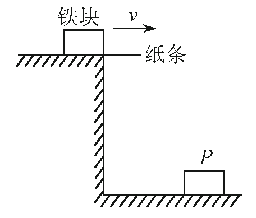
\includegraphics[width = 0.3\textwidth]{images/momentum-1.pdf} 
	\end{flushright}
\tagged{student}{\vspace*{1cm}}
\begin{taggedblock}{teacher}
\noindent
解析:B
%当以速度$2v$抽出纸条时,摩擦力作用的时间变短,根据动量定理铁块的速度将比之前更小,所以将会落在$P$点的左边。
%在教学中可以将一张纸放在板擦下抽出演示这个过程,让学生可以自己尝试,以便活跃课堂气氛。

\end{taggedblock}
\end{example}
%%%%%%%%%%%%%%%%%%%%%%%%%%




\begin{example}
一个质量$m=2\unit{kg}$的物体,在$F_1 = 8\unit{N}$的水平力作用下从静止开始沿水平面运动了$t_1 = 5\unit{s}$,然后推力减小为$F_2 = 5\unit{N}$,方向不变,物体又运动了$t_2=4\unit{s}$后撤去外力,物体再经过$t_3 = 6\unit{s}$后停下来。
试求物体在水平面上所受的摩擦力。
%\begin{flushright}
%\includegraphics[width = 0.3\textwidth]{images/.pdf} 
%\end{flushright}
\tagged{student}{\vspace*{4cm}}
\begin{taggedblock}{teacher}
\noindent
解析:4N
\end{taggedblock}
\end{example}




\subsection{多个物体的运动}
如果动量定理只能够应用到上面这些简单的问题实际上就没有提出它的必要了。
如果一个力学系统包含多个物体,它们除了受到外力作用彼此之间还有内力作用,根据牛顿第三定律,所有的内力均大小相等、方向相反并且在同一条直线上。
假设各个物体的质量和速度分别为$m_i$和$v_i$,对于第$i$个物体它所受到的合力可以分解为两部分,一部分来自于系统之外而另一部分则是该力学系统内部其它物体对它的作用力:
\begin{equation}
\vec{F}_i = \vec{F}_i^{(e)}+\sum_{j\neq i}^{N}\vec{f}_{ji}
\end{equation}
其中求和是针对力学系统内除第$i$个物体以外的物体进行的,内力$f_{ji}$代表第$j$个物体对第$i$个物体的力,根据牛顿第三定律我们知道
\begin{equation}
f_{ji} = -f_{ij},
\end{equation}
这样在一小段时间$\Delta t$内对第$i$个物体应用动量定理
\begin{equation}
F_i\Delta t = \Delta p_i,
\end{equation}
将上式对系统内所有的质点求合并且利用牛顿第三定律我们可以得到
\begin{equation}
\big(\sum_{i=1}^{N}F_i^{e}\big) \Delta t = \Delta \big(\sum_{i=1}^{N}p_i\big)
\end{equation}
上式中左边为所有外力在给定时间内的冲量,而右边则是力学系统的总动量在给定时间间隔内的变化量。
也就是说一个力学系统总动量的变化量只与所有外力的冲量有关,无论内力的形式多么复杂都不影响总动量的变化。


%%%%%%%%%%%%%
\begin{example}
	两个质量分别为$m_1$和$m_2$的物体由弹性系数为$k$,原长为$l_0$的弹簧连接,初始时刻弹簧状态未知,初始时刻整个系统竖直放置。
	现让系统下落,已知下落时间为$t$时质量为$m_1$的物体向下运动速度为$v_1$,求另一物体的速度$v_2$。
	\tagged{student}{\vspace*{4cm}}
	\begin{taggedblock}{teacher}
	\newline
		解析:$(m_1+m_2)gt=m_1v_1+m_2v_2$
	\end{taggedblock}
\end{example}
%%%%%%%%%%%%%%%%%%%%


%%%%%%%%%%%%%%%%%%%%%%%%%%%%%%%%%%
\begin{example}
如图,$A$、$B$两小物体被平行于斜面的轻细线相连,均静止于斜面上。
以平行与斜面向上的恒力拉$B$,使两物体同时由静止起以加速度$a$沿斜面向上运动。
经时间$t_1$,细线突然被拉断。
再经时间$t_2$,$A$上滑到它能达到的最高点。
已知A、B的质量分别为$m_A$和$m_B$,细线断后拉$B$的恒力保持不变,求$A$到达最高点时$B$的速度。
	\begin{flushright}
		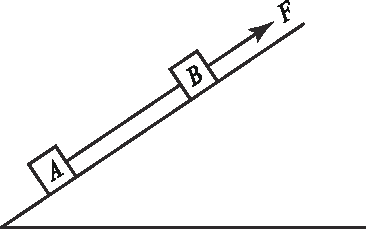
\includegraphics[width = 0.3\textwidth]{images/momentum-2.pdf} 
	\end{flushright}
\tagged{student}{\vspace*{4cm}}
\begin{taggedblock}{teacher}
\noindent
解析:$(m_A+m_B)a=F  F*(t_1+t_2)=m_B*v$
\end{taggedblock}
\end{example}
%%%%%%%%%%%%%%%%%%%%%%%%%%

%%%%%%%%%%%%%%%%%%%%%%%%%%%%%%%%%%%%%%%
\begin{example}
光滑地面上一个箱子A质量$m_A = 2\unit{kg}$,以初速度$v_0 = 10\unit{m/s}$冲向静止的箱子B,B的质量为$m_B=1\unit{kg}$,碰完后
\begin{enumerate}
\item 如果A的速度变成了5\unit{m/s},则B的速度为多少?
\item 如果A、B之间由于涂了强力胶水一碰就沾上了,则合体后速度为多少?
\end{enumerate}
\begin{flushright}
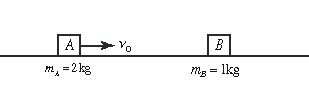
\includegraphics[width=0.4\textwidth]{images/momentum-problem-1.pdf}
\end{flushright}
\tagged{student}{\vspace*{4cm}}
\begin{taggedblock}{teacher}
\noindent
解析:1.$10m/s$ $20/3 m/s$
\end{taggedblock}
\end{example}


\subsection{冲击和碰撞}
原则上只要我们始终清楚作用在物体上力的大小和方向时,应用动量定理和牛顿定律都可以得到相同的结果。
对于某有些物理过程,无论我们多么努力都没法判断或测量各个时刻的作用力,反而物体受力前后运动的变化却很容易确定。
冲击和碰撞就是具有这种特点的物理过程,两个坚硬物体的碰撞时间极短,相互作用力极大并且变化方式极其复杂,但是碰撞前后速度的变化却很容易测量,也就是说碰撞力的大小和作用时间很难确定,但是碰撞力的冲量则容易得到。
因为时间极短,所以在碰撞或冲击过程中除了碰撞力以外的其它外力,如重力、摩擦力、弹簧力等都可以忽略不计,在碰撞的瞬间所产生的运动变化可以认为完全由冲击力导致。
当物体受到给定冲量后的动量变化可以由动量定理\ref{eq: 动量定理的微分形式}给出,相互碰撞的两个物体所受到的冲量大小相等、方向相反。

我们可以根据力学系统的特点决定各个物体所受到的冲击:




\begin{example}
如图所示,三个小球ABC的质量都为$m$,放于光滑的水平桌面上,三球之间各用质量忽略的不可伸长的绳相连,ABC夹角为 $120\degree$。
现沿BA绳方向给A一个瞬时冲量$I$,求C球获得的速度为多少?
\begin{flushright}
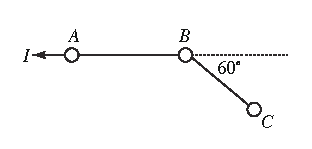
\includegraphics[width=0.3\textwidth]{images/momentum-problem-2.pdf}\end{flushright}
\tagged{student}{\vspace*{4cm}}
\begin{taggedblock}{teacher}
\noindent
解析:$\frac{2I}{15m}$
在解完题之后,如果有时间可以向学生解释绳、杆、面等不同情况下冲量的性质和方向。


也可以根据力的性质导出不同方向冲击力冲量的关系
\end{taggedblock}
\end{example}



%%%%%%%%%%%%%%%%%
\begin{example}

军训时,战士距离$s_0$以速度$v_0$起跳,再用脚蹬墙一次,使身体变为竖直向上的运动以继续升高,墙面与鞋底之间的摩擦系数为$\mu$,求能使人体重心有最大总升高的起跳角度。
\tagged{student}{\vspace*{4cm}}
\begin{taggedblock}{teacher}
\newline
解析:
$\arctan\theta=\mu$可用图像法解题。用脚蹬墙一次,竖直方向上的速度加了$v_0\cos\theta*\mu$。作出速度-时间图像,面积就是上升的高度。
\\
拓展:当$\arctan\theta=\frac{v_0^2}{g}$时,到达墙面的时候有最大的高度,但是若需要求总升高的最高,则需要$\frac{v_0^2\sin^2\theta}{2g}+\frac{\mu^2v_0^2\cos^2\theta}{2g}+\frac{\mu v_0\cos\theta}{g}*(v_0\sin\theta-\frac{s_og}{v_0\cos\theta})$达到最大
\end{taggedblock}
\end{example}
%%%%%%%%%%%%%%%%%%%%%%


\begin{example}
在光滑水平面上有两面相距为$d$平行的墙面,有一个旋转的球撞向其中一个竖直墙壁,如果墙壁为光滑时,在经过弹性碰撞后球垂直于墙的速度分量反向,平行于墙的分量保持不变。
假设弹性碰撞之后球最终击中对面墙壁上的A点。
如果球的墙之间的摩擦系数为$\mu$,假设经墙壁反弹后小球垂直于墙壁的速度大小不变、方向相反,求证在反弹之后在另一面墙壁上的落点与A点的距离同小球的初始位置、初速度的方向均无关。

\begin{flushright}
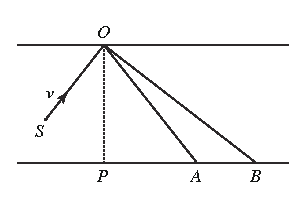
\includegraphics[width = 0.3\textwidth]{images/momentum-problem-3.pdf} 
\end{flushright}
\tagged{student}{\vspace*{4cm}}
\begin{taggedblock}{teacher}
\noindent
解析:略
\end{taggedblock}
\end{example}

\subsection{应用到流体}
动量定理的另一个有威力的应用是在处理和流体有关的问题中。
假设一种流体介质由数目极大的分子构成,每个分子的质量均为$m$,单位体积内有$n$个分子,而每个分子都处于静止状态。
考察一个截面积为$S$的长条形物体在该介质中沿着其轴线方向以速度$v$做运动,它可以吸附其截面上所有的介质分子。
在$\Delta t$微小时刻之中,它可以吸附$S\cdot v\Delta t$体积内所有的介质分子,每个分子得到了和飞船一样的速度。
以所有吸附的介质分子为研究对象,$\Delta t$时间时它们的动量变化
\begin{equation}
n  S v \Delta t\cdot mv = nmSv^2\Delta t = \rho S v^2\Delta t,
\end{equation}
其中$\rho$为介质的密度。
根据动量定理我们知道它们在$\Delta t$时间内受到的冲量就是上式给出的动量变化,与此同时牛顿第三定律告诉我们介质分子会飞船的冲量大小与上式相同,方向则是与速度方向相反。
可以把这样的冲量看做是一个恒力的作用,表现为在该介质中运动的飞船所受到的阻力,很明显飞船受到的阻力
\begin{equation}
F = \frac{\Delta I}{\Delta t} =  \rho S v^2.
\end{equation}
可以看出阻力正比于介质的密度,介质中运动物体的横截面与速度的平方。

需要特别强调的是以这种方法求出微观颗粒对宏观物体的作用力的问题当中,单个微观粒子与宏观物体碰撞的行为会影响到宏观力的大小和方向。



\begin{example}
和前面的例子相同,但是介质粒子在碰撞之后以相同的相对速度反弹,求在这种情况下飞船受到的阻力。
%\begin{flushright}
%\includegraphics[width = 0.3\textwidth]{images/.pdf} 
%\end{flushright}
\tagged{student}{\vspace*{4cm}}
\begin{taggedblock}{teacher}
\newline
解析:$2 \rho S v^2$
\end{taggedblock}
\end{example}

\begin{example}
如果飞船的外形可以假设为一个角度为$\alpha$,长度为$L$的圆锥形,和介质粒子的碰撞同样是弹性,求此时飞船受到的阻力。
%\begin{flushright}
%\includegraphics[width = 0.3\textwidth]{images/.pdf} 
%\end{flushright}
\tagged{student}{\vspace*{4cm}}
\begin{taggedblock}{teacher}
\newline
解析:$2 \rho v^2(1-\cos\alpha)\frac{L^2\pi}{\tan^2\frac{\theta}{2}}$
\end{taggedblock}
\end{example}


%%%%%%%%%%%%%%%%%
\begin{example}
一帆船在静水中顺风航行,风速为$v_0$。
假设帆面是完全弹性面,风与帆面垂直时求船速多大时风供给船的功率为最大?

\tagged{student}{\vspace*{4cm}}
\begin{taggedblock}{teacher}
\noindent
解析:$\frac{v_0}{2}$
\end{taggedblock}
\end{example}
%%%%%%%%%%%%%%%%%%%%%%

\begin{example}
近代物理认为光线是由光子构成,光子的动量与光子能量的关系为$E = pc$,其中$c$为光速。
假设太阳的功率为$P_S$,试求在距离太阳为$r$处受到太阳辐射的光子冲击所产生的压强。
%\begin{flushright}
%\includegraphics[width = 0.3\textwidth]{images/.pdf} 
%\end{flushright}
\tagged{student}{\vspace*{4cm}}
\begin{taggedblock}{teacher}
\newline
解析:量级为$\frac{P_s}{4\pi r^2c}$
\end{taggedblock}
\end{example}




\subsection{质量变化的情况}
一辆行驶的汽车会不断在消耗它的汽油,飞行的飞机或火箭也有同样的特点,它们在运动过程中质量总是不断变化的。
可以将动量定理运用到这类问题,在微小时间$\Delta t$中设物体受到冲量$\Delta I$,而同样时间里的动量变化可以分解为速度的变化和质量的变化:
\begin{equation}
\Delta I = \Delta p = \Delta (mv) = \Delta m\cdot v+m\cdot \Delta v
\end{equation}
结合实际性况得到质量变化的方式以后就可以进一步得出运动的其它性质。

\begin{example}
在雨中用恒力$F$去推一个质量为$M$,截面积为$S$容器,假设一个静止在地面的容器单位时间水位的高度上升$\Delta h$,不考虑雨水对容器前方的阻力,水的密度为$\rho$求在3单位时间后容器的速度。
%\begin{flushright}
%\includegraphics[width = 0.3\textwidth]{images/.pdf} 
%\end{flushright}
\tagged{student}{\vspace*{4cm}}
\begin{taggedblock}{teacher}
\newline
解析:$V=\frac{3F}{M+3S\rho\Delta h}$
\end{taggedblock}
\end{example}



%%%%%%%%%%%%%%%%%
\begin{example}

长度为$l$,质量为$m$的柔软绳子放在水平桌面上,用手将绳子的一端以恒定的速度$v$向上提起,求当提起高度为$x(x<l)$时手的提力。
\tagged{student}{\vspace*{4cm}}
\begin{taggedblock}{teacher}
\newline
解析:$\frac{mv^2}{l}+\frac{mgx}{l}$
\end{taggedblock}
\end{example}
%%%%%%%%%%%%%%%%%%%%%%

\begin{example}
如图所示一质量为$m$,长为$l$的柔软绳自由悬垂,下端恰与一台秤盘接触。
某时刻放开柔软绳上端,求台称在任意时刻的读数以及读数的最大值。
	\begin{flushright}
		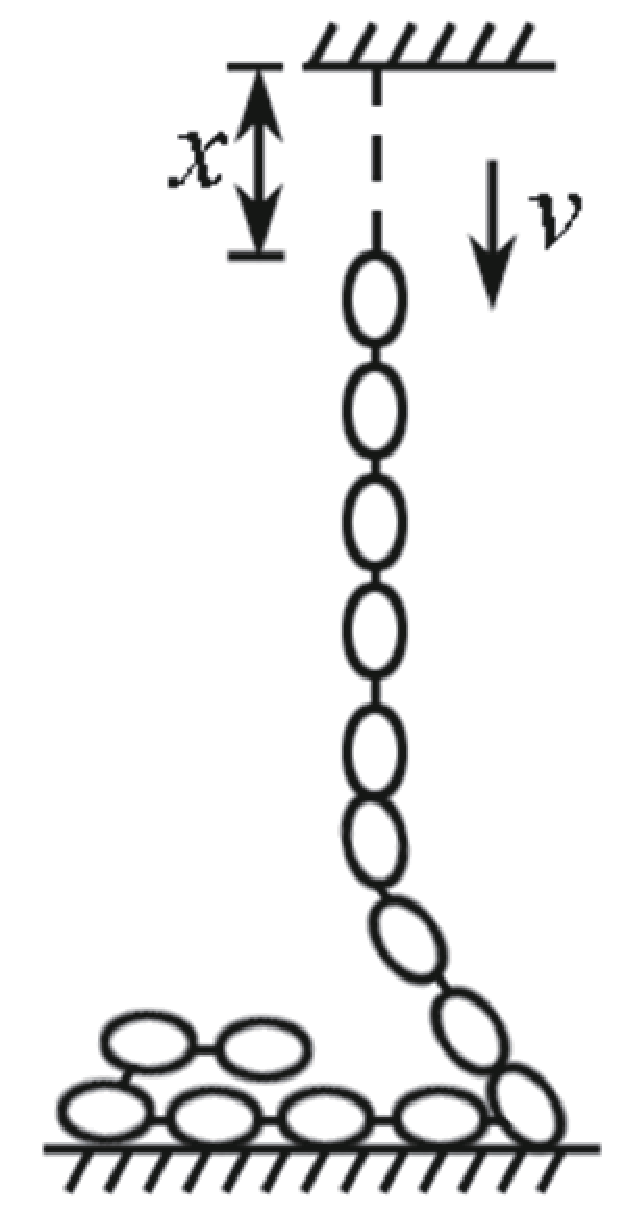
\includegraphics[width = 0.2\textwidth]{images/momentum-3.pdf} 
	\end{flushright}
%\begin{flushright}
%\includegraphics[width = 0.3\textwidth]{images/.pdf} 
%\end{flushright}
\tagged{student}{\vspace*{2cm}}
\begin{taggedblock}{teacher}
\noindent
解析:$F=\frac{3mg^2t^2}{2l}$ $F_MAX=3mg$
\end{taggedblock}
\end{example}

\begin{example}
假设在某一密度为$\rho$的均匀介质中下落的截面积为$S$的物体由于吸附介质引起的质量变化不能忽略不计,如果它能够吸附所有与之相遇的介质分子,试给出该物体速度和质量随时间变化的方程,不要求求解,但需要定性分析该物体的运动。
%\begin{flushright}
%\includegraphics[width = 0.3\textwidth]{images/.pdf} 
%\end{flushright}
\tagged{student}{\vspace*{4cm}}
\begin{taggedblock}{teacher}
\newline
解析:$(m(t)+\rho Sv\Delta t)(v(t)+\Delta t)=0$
\end{taggedblock}
\end{example}

\begin{example}
球状小水滴在静止的雾气中下落,下落过程中吸附了全部所遇到的水分子。
设水滴始终保持球状,设雾气密度均匀,忽略空气阻力,重力加速度取恒定值$g$。
试列出水滴下落过程中它的质量、速度、半径所满足的方程,并定性分析水滴的运动,不要求求解运动方程。
%\begin{flushright}
%\includegraphics[width = 0.3\textwidth]{images/.pdf} 
%\end{flushright}
\tagged{student}{\vspace*{4cm}}
\begin{taggedblock}{teacher}
\newline
解析:$(Sv\Delta t\rho+m)(v+\Delta v)=mg\Delta t$   $v=\frac{4\pi R^3}{3}$ $S=\pi R^2$
\end{taggedblock}
\end{example}






\section{动量守恒}
前面我们学过了动量定理以及它的各种应用。
动量定理告诉我们,一个受到外力作用的力学系统在一段过程前后的动量变化等于外力在该过程中的总冲量,与内力无关。
一个直接的推论就是如果一个力学系统所受的外力为零时,运动前后的动量变化为零,也就是我们常说的动量守恒。
在实际使用当中动量守恒有以下几种典型的表现形式
\begin{description}
\item[孤立系统]
如果一个力学系统不受任何外力的作用则称之为一个孤立的力学系统。
毫无疑问孤立的力学系统总动量必然是守恒的,因为动量是一个矢量,所以动量守恒会给我们提供三个独立的方程,用来表达在三个独立的方向上任意一个时间点的动量均与初动量相同。
\item[分动量守恒]
真正孤立的力学系统原则上是不存在的,但是如果在一个问题当中所考察的对象在某些特定的方向上所受合外力为零,那么在这些方向上的分动量守恒,尽管其它方向上的动量会发生变化。
\item[碰撞瞬间的动量守恒]
对于在极短时间受到极大冲击力而导致的冲击或碰撞过程,因为其它作用力在这样如此短的时间里产生的冲量与冲击力相比极其小,可以忽略不计。
所以可以近似地认为在这样的物理过程当中碰撞前后的总动量近似保持不变。
\end{description}

动量守恒虽然是动量定理的特殊情况,但是却包含着非常丰富的内容,帮助我们处理很多有用的物理问题。



\subsection{总动量守恒}
因为自然界的物体总是处于复杂的相互作用环境当中,所以严格意义上的孤立系统是不存在的,但是如果一个力学系统和其它对象之间的相互作用极其微弱的话,可以将它近似地看做是一个孤立系统。
一个力学系统能否看成孤立系统与在给定问题中计算的精度有关,比如地球和月球构成的系统在一定程度上就可以看做是一个孤立系统,但是太阳对地月系统的作用力在有些问题中就非常明显,这时就必须认真考虑太阳的存在。
如果一个力学能够看做是孤立系统的话,它的总运动量的三个分量分别守恒,与内力的形式的大小均无关系。


%%%%%%%%%%%%%%%%%
\begin{example}

地球和所有地球上的物体可以看成是是近似的孤立系统,理应有动量守恒。
而当一个人从地面上跳起时他的动量发生了改变,如何解释这一现象。
\tagged{student}{\vspace*{4cm}}
\begin{taggedblock}{teacher}
\newline
解析:地球也动了,但是质量相差悬殊,几乎感觉不到。
\end{taggedblock}
\end{example}
%%%%%%%%%%%%%%%%%%%%%%



\subsection{动量的分量守恒}

孤立系统的动量守恒定律的应用范围极其狭窄,很明显这是由于真实孤立的体系实际上是不存在的,自然界中各个物体之间都存在有广泛的相互作用。
但注意到动量本身是一个矢量,空间中的动量定理实际上由三个独立的方程构成,在给定的物理过程中,当在某个特定方向上的合外力为零时,系统的总动量在这个方向上的分量实际上在运动过程中依然保持不变,这就是动量守恒的分量形式。




%%%%%%%%%%%%%%%%%
\begin{example}

在水平面上有多个物体构成的系统,它们与水平面之间均无摩擦力,在开始一时刻它们均处于静止状态。
求证在此后的运动过程中,系统质心位置保持不变。

\tagged{student}{\vspace*{4cm}}
\begin{taggedblock}{teacher}
\noindent
解析:略
\end{taggedblock}
\end{example}
%%%%%%%%%%%%%%%%%%%%%%



%%%%%%%%%%%%%%%%%
\begin{example}

如图所示,两根长度均为$l$,质量可忽略不计的轻杆,一端通过质量为$m$的球形铰链连接,另一端分别接有质量为$m$和$2m$的小球。
将此装置两杆并拢,铰链向上放在桌上,然后轻敲一下使球向两边滑,两杆保持在竖直平面内,所有摩擦均忽略不计。
建立如图所示的坐标系,初始时刻位于$x=0$处,求两杆夹角为$90^\circ$以及完全展开成水平状态时质量为$2m$小球的位置。
	\begin{flushright}
		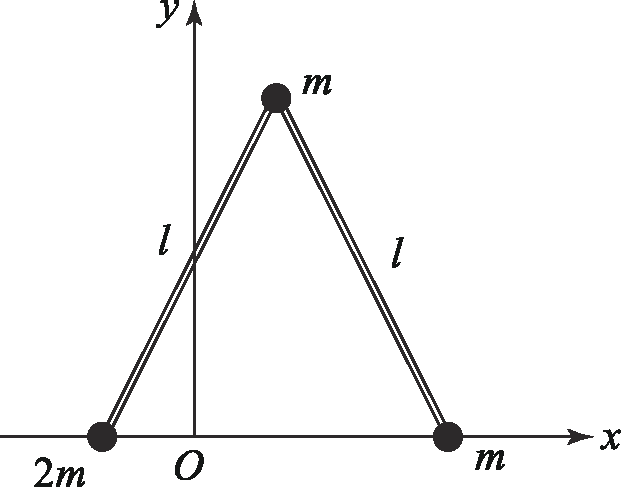
\includegraphics[width = 0.3\textwidth]{images/momentum-4.pdf} 
	\end{flushright}
\tagged{student}{\vspace*{4cm}}
\begin{taggedblock}{teacher}
\noindent
解析:$x=-\frac{3\sqrt{2}l}{8}$     $x=-\frac{3l}{4}$
\end{taggedblock}
\end{example}
%%%%%%%%%%%%%%%%%%%%%%



\subsection{冲击、碰撞过程中的动量守恒}


%%%%%%%%%%%%%%%%%
\begin{example}

一个质量为$M$的质点$A$由距离水平面高$H$的地方从静止开始自由下落,当它下落到高度为$h$的地方时,被一颗质量为$m$,沿水平方向以速度$v$飞行的子弹击中,子弹与$A$碰撞时间极短并最终停留在该物体内部,求$A$落地点与未被击中时下落点的距离$l$。 
	\begin{flushright}
		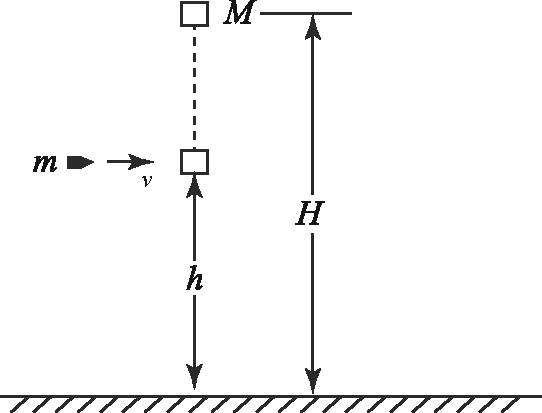
\includegraphics[width = 0.4\textwidth]{images/momentum-5.pdf} 
	\end{flushright}
\tagged{student}{\vspace*{3cm}}
\begin{taggedblock}{teacher}
\noindent
解析:碰撞后水平速度和竖直速度都会变,水平速度变成$\frac{mv}{M+m}$ 竖直速度变成$\frac{M\sqrt{2(H-h)}}{m+M}$,之后做加速度为g的曲线运动。
\end{taggedblock}
\end{example}
%%%%%%%%%%%%%%%%%%%%%%






\subsection{质心参考系}
动量守恒定律不仅可以帮助我们计算在不受外力(或某些特定方向不受外力)的力学系统给定运动前后的动量,还有很多推论,这其中最重要的就是动量守恒的力学系统质心的运动规律了。
考虑一个由多个质点构成的力学系统,由$N$个质量分别为$m_i$的质点构成,第$i$个质点的位置由矢量$x_i$来表示,那么该系统的质心位置$x_C$为
\begin{equation}\label{eqn: 力学系统质心的定义}
x_C = \frac{\sum_{i=1}^N m_ix_i}{\sum_{i=1}^N m_i}
\end{equation}
与此同时系统的总动量则是
\begin{equation}
p = \sum_{i=1}^N m_i v_i = \sum_{i=1}^Nm_i\frac{\Delta x_i}{\Delta t}=\frac{\Delta}{\Delta t}\left(\sum_{i=1}^N m_i x_i \right) = M \frac{\Delta x_C}{\Delta t}
\end{equation}
其中$M=\sum_{i=1}^N m_i$,为所有质点的质量和,并且利用了质心定义\ref{eqn: 力学系统质心的定义}。
从中可以看出总动量不但可以表达成各个质点的动量的矢量和,还可以表达成系统总质量$M$与质心速度$v_C = \frac{\Delta x_C}{\Delta t}$的乘积。
如果系统的动量守恒,那么任何时间的总动量不随时间而变,是一个常数。
这样我们可知,对于动量守恒的力学系统来说它的质心速度保持不变,也就是说不受外力作用的系统质心或者静止,或者做匀速直线运动,与初始时刻质心的运动状态有关。

%%%%%%%%%%%%%
\begin{example}
	两个质量分别为$m_1$、$m_2$的质点由劲度系数为$k$,原长为$l_0$的轻弹簧连接。
	开始时刻将弹簧拉长到$l>l_0$静止释放,在此后的运动过程中弹簧上是否存在有一点,它的位置始终保持不变?
	\tagged{student}{\vspace*{4cm}}
	\begin{taggedblock}{teacher}
		\newline
		解析:存在,就是它的质心
	\end{taggedblock}
\end{example}
%%%%%%%%%%%%%%%%%%%%


%%%%%%%%%%%%%
\begin{example}
	一个质量为$M$、半径为$R$的球形碗放在光滑水平面上,另一个质量为$m$的质点$A$开始时位于碗的边缘静止释放,求$A$在下落过程以地面为参考系中的运动轨迹。
		\begin{flushright}
			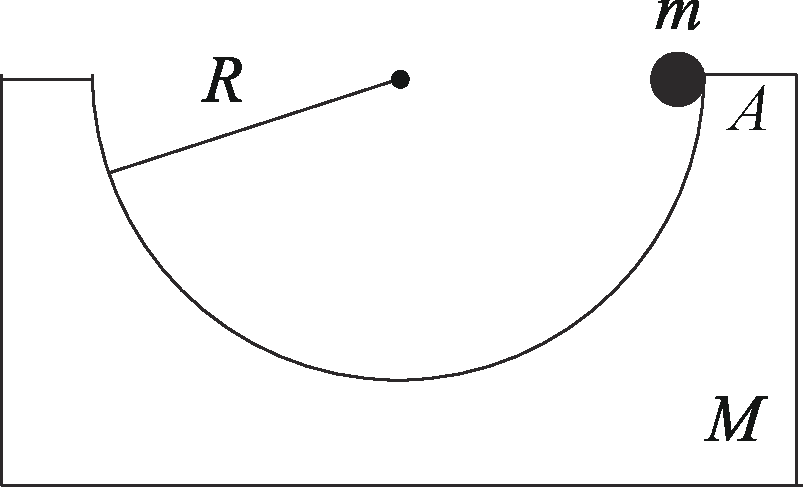
\includegraphics[width = 0.3\textwidth]{images/momentum-6.pdf} 
		\end{flushright}
	\tagged{student}{\vspace*{4cm}}
	\begin{taggedblock}{teacher}
		\noindent
		解析:椭圆,长半轴为R,短半轴为$\frac{MR}{m+M}$
	\end{taggedblock}
\end{example}
%%%%%%%%%%%%%%%%%%%%

把整个太阳系看做一个孤立的力学系统是一个极好的近似,由于太阳的质量远远大于太阳系中其它行星的质量,所以太阳可以看做是近似不动的。
但是如果认真考虑其它行星的质量时在相互作用过程中太阳位置的变化也不能忽略不计。


另外一个力学系统的运动变化仅由内力引起的话,它的质心的运动与先前的运动完全相同。
看以下几个例子:




 


\section{变质量系统,火箭}
火箭是依靠从其尾部喷出高温高压的,由燃料燃烧所产生气体而获得巨大推力最终克服地球引力使航天器飞向太空工具,随着技术的进步,火箭的推力越来越大。
火箭的升空过程极其复杂,为简单起见我们假设火箭沿着一条直线运动并且忽略重力,简单的分析可知在喷气过程中火箭和喷出气体构成的系统由于只有内力作用所以动量守恒,但是随着气体逐渐被喷出,火箭的质量也在不断地发生变化,这时我们无法简单地应用动量守恒定律来推测火箭速度与喷出气体质量的关系。
但是如果我们考察一小段时间$\Delta t $,在此期间火箭以相对于箭体$u$的速度向后喷出一定质量的气体,从而获得了反冲。
建立一个正方向为火箭运动方向的坐标系,假设在喷气之前火箭的质量为$M$,在$\Delta t$时间里喷气后火箭的质量产生了$\Delta M$的变化,这样火箭的质量变成了$M+\Delta M$,由于反冲效应,其速度为原先的$v$变成了$v+\Delta v$。
需要特别指出的是$\Delta M<0$,这样的选择是因为我们更关注火箭质量的变化,而对喷出气体的质量以及速度则兴趣不大。

根据上面的约定,火箭实际上喷出了$-\Delta M$的气体,在给定的坐标系中气体相对于地面的速度为$v-u$,这样动量守恒定律将给出:
\[
Mv = (M+\Delta M)(v+\Delta v)-\Delta M(v-u),
\]
将上式展开并化简可得
\[
M\Delta v + u\Delta M +\Delta M\Delta v = 0.
\]
如果$\Delta t$选得足够小,使得在如此之短的时间里,火箭质量和速度的变化量与火箭自身的质量和速度相比极其之小的话,上式左边第三项实际上可以忽略不计,这样我们就得到了火箭速度的增量$\Delta v$与喷出气体的质量$-\Delta M$以及速度$u$的一个关系:
\begin{equation}\label{eqn: momentum: rockey}
\Delta v = -u\frac{\Delta M}{M},
\end{equation}
这就是简化了的火箭模型在升空过程中所满足的方程,
从中可以清楚地看到火箭质量的减小与速度增加量之间的关系。

%%%%%%%%%%%%%
\begin{example}
	在火箭升空过程中某一时刻它的质量为$M$,速度为$v$,喷气相对速度为$u$,忽略地球引力,请根据方程\ref{eqn: momentum: rockey}在下面坐标系中定性地画出此后火箭的速度与质量的关系。
	\tagged{student}{\vspace*{4cm}}
	\begin{taggedblock}{teacher}
	\newline
		解析:略
	\end{taggedblock}
\end{example}
%%%%%%%%%%%%%%%%%%%%

%%%%%%%%%%%%%
\begin{example}
	火箭在未发射时的质量为$M_0$,在烧完所有燃料之后的质量为$M$,简单起见设这是一个单级火箭,喷气速度为$u$,试证明最终火箭的速度
	\[v = u\ln\frac{M_0}{M}\]
	\tagged{student}{\vspace*{4cm}}
	\begin{taggedblock}{teacher}
		\newline
		解析:略
	\end{taggedblock}
\end{example}
%%%%%%%%%%%%%%%%%%%%














